% !TEX encoding = UTF-8
% !TEX TS-program = pdflatex
% !TEX root = ../tesi.tex

\subsection{UC3 - Visualizzazione dati ordinati per file}
\begin{itemize}
  \item \textbf{Identificativo}: UC3
  \item \textbf{Nome}: visualizzazione dati ordinati per file
  \item \textbf{Descrizione grafica}:
\end{itemize}

\begin{figure}[h]
  \centering
  %  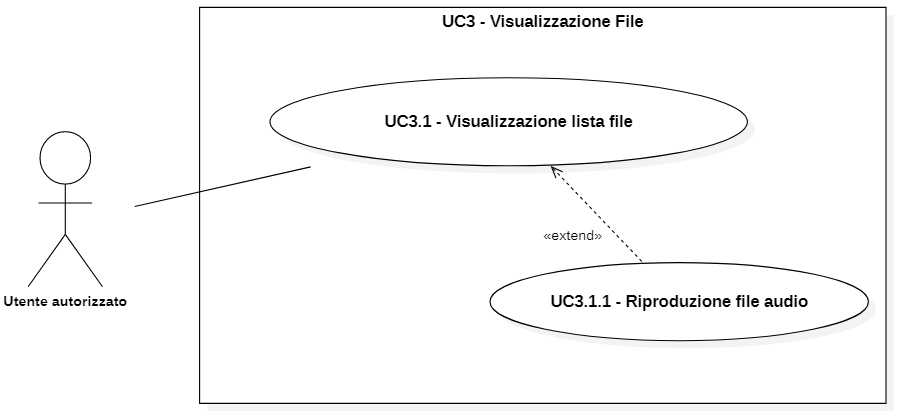
\includegraphics[scale=0.50]{images/UC3.png}
  \caption{Descrizione grafica caso d'uso UC3}
\end{figure}

\begin{itemize}
  \item \textbf{Attori}
        \begin{itemize}
          \item \textit{Primari}: utente autorizzato
        \end{itemize}
  \item \textbf{Precondizione}: l'utente si trova sulla pagina per il caricamento dati, che ha già effettuato correttamente.
  \item \textbf{Postcondizione}: l'utente visualizza i dati caricati sull'applicazione, ordinati per nome dei file.
  \item \textbf{Scenario principale}: l'utente ha caricato correttamente i dati e questi vengono visualizzati ordinati per nome del file.
\end{itemize}
\newpage